% !TeX spellcheck = en_GB
% !TeX program = pdflatex
%
% LuxSleek-CV 1.1 LaTeX template
% Author: Andreï V. Kostyrka, University of Luxembourg
%
% 1.1: added tracking and letter-spacing for prettier lower caps, added `~` for language levels
% 1.0: initial release
%
% This template fills the gap in the available variety of templates
% by proposing something that is not a custom class, not using any
% hard-coded settings deeply hidden in style files, and provides
% a handful of custom command definitions that are as transparent as it gets.
% Developed at the University of Luxembourg.
%
% *NOTHING IS HARCODED, and never should be.*
%
% Target audience: applicants in the IT industry, or business in general
%
% The main strength of this template is, it explicitly showcases how
% to break the flow of text to achieve the most flexible right alignment
% of dates for multiple configurations.

\documentclass[11pt, a4paper]{article}

\usepackage[T1]{fontenc}     % We are using pdfLaTeX,
\usepackage[british]{babel}
\usepackage[left = 0mm, right = 0mm, top = 0mm, bottom = 0mm]{geometry}
\usepackage{graphicx}        % To insert pictures
\graphicspath{ {./images/} }
\usepackage{xcolor}          % To add colour to the document
\usepackage{marvosym}        % Provides icons for the contact details
\usepackage{fontawesome5}
\usepackage{enumitem}        % To redefine spacing in lists
\setlist{parsep = 0pt, topsep = 0pt, partopsep = 1pt, itemsep = 1pt, leftmargin = 6mm}

\usepackage{fontspec,xltxtra,xunicode}
\defaultfontfeatures{Mapping=tex-text}
\setmainfont[Ligatures=TeX]{Times New Roman}
\setromanfont[Mapping=tex-text]{Times New Roman}
\renewcommand{\familydefault}{\sfdefault}

\definecolor{cvblue}{HTML}{304263}

%%%%%%% USER COMMAND DEFINITIONS %%%%%%%%%%%%%%%%%%%%%%%%%%%
% These are the real workhorses of this template
\newcommand{\dates}[1]{\hfill\mbox{\textbf{#1}}} % Bold stuff that doesn’t got broken into lines
\newcommand{\is}{\par\vskip.5ex plus .4ex} % Item spacing
\newcommand{\smaller}[1]{{\small$\diamond$\ #1}}
\newcommand{\headleft}[1]{\vspace*{3ex}\textsc{\textbf{#1}}\par%
\vspace*{-1.5ex}\hrulefill\par\vspace*{0.7ex}}
\newcommand{\headright}[1]{\vspace*{2.5ex}\textsc{\Large\color{cvblue}#1}\par%
\vspace*{-2ex}{\color{cvblue}\hrulefill}\par}
%%%%%%%%%%%%%%%%%%%%%%%%%%%%%%%%%%%%%%%%%%%%%%%%%%%%%%%%%%%%

\usepackage[colorlinks = true, urlcolor = white, linkcolor = white]{hyperref}

\begin{document}

% Style definitions -- killing the unnecessary space and adding the skips explicitly
    \setlength{\topskip}{0pt}
    \setlength{\parindent}{0pt}
    \setlength{\parskip}{0pt}
    \setlength{\fboxsep}{0pt}
    \pagestyle{empty}
    \raggedbottom

    \begin{minipage}[t]{0.33\textwidth} %% Left column -- outer definition
%  Left column -- top dark rectangle
        \colorbox{cvblue}{\begin{minipage}[t][5mm][t]{\textwidth}
                              \null\hfill\null
        \end{minipage}}

        \vspace{-.2ex} % Eliminates the small gap
        \colorbox{cvblue!90}{\color{white}  %% LEFT BOX
        \kern0.09\textwidth\relax% Left margin provided explicitly
            \begin{minipage}[t][293mm][t]{0.82\textwidth}
                \raggedright
                \vspace*{2.5ex}

                \Large Hugo \textbf{\textsc{Gonçalves}} \normalsize

% Centering without extra vertical spacing
                \null\hfill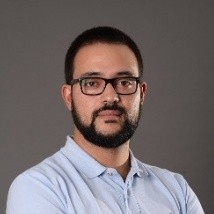
\includegraphics[width=0.65\textwidth]{hg}\hfill\null

                \vspace*{0.5ex} % Extra space after the picture

                \headleft{Profile}
                \textbf{Software Engineer} with over eight years of dedicated experience in crafting distributed, real-time and high-performance backend systems.


                \headleft{Contact details}
                \small % To fit more content
                \MVAt\ {\small \href{mailto:email@hugogoncalves.pt}{email@hugogoncalves.pt}} \\[0.4ex]
                \Mobilefone\ +351\,91\,00\,41\,754 \\[0.5ex]
                \faGithub\ \href{https://github.com/goncah}{github.com/goncah} \\[0.1ex]
                \Mundus\ \href{https://hugogoncalves.pt}{hugogoncalves.pt} \\[0.1ex]
                \faLinkedin\ \href{https://linkedin.com/in/goncalh}{linkedin.com/in/goncalh} \\[0.1ex]
                \faOrcid\ \href{https://orcid.org/0009-0007-5803-4499}{orcid.org/0009-0007-5803-4499} \\[0.1ex]
                \normalsize

                \headleft{Personal information}
                Citizenship: \textbf{Portuguese} \\[0.5ex]
                Languages: \textbf{Portuguese}~(native), \textbf{English}

                \headleft{Skills}
                \begin{itemize}
                    \item Java, Java EE, Jakarta EE
                    \item Apache Kafka, Kafka Streams, Kafka Connect, AWS MSK
                    \item Springboot, Helidon
                    \item Wildfly
                \end{itemize}

            \end{minipage}%
            \kern0.09\textwidth\relax%%Right margin provided explicitly to stretch the colourbox
        }
    \end{minipage}% Right column
    \hskip2.5em% Left margin for the white area
    \begin{minipage}[t]{0.56\textwidth}
        \setlength{\parskip}{0.8ex}% Adds spaces between paragraphs; use \\ to add new lines without this space. Shrink this amount to fit more data vertically

        \vspace{2ex}

        \headright{Experience}

        \textsc{Software Engineer} at \textit{Vodafone Group.}  \dates{2024.05--present} \\
        \smaller{Real-time payments fraud detection with Kafka, Kafka Streams and Java 21, Charging \& Payments integration with Springboot microservices.}

        \is
        \textsc{Software Engineer} at \textit{Vodafone Group.}  \dates{2023.04--2024-04} \\
        \smaller{Ticketing, Inventory and Network Management systems integration API development with Java 17, Jakarta EE, Wildfly.}

        \is
        \textsc{Software Engineer} at \textit{Vodafone Group.}  \dates{2018.07--2023-03} \\
        \smaller{Workflow process development with Java 8 for the mobile network automation platform.}

        \is
        \textsc{Software Engineer} at \textit{Vodafone Group.}  \dates{2016.06--2018-06} \\
        \smaller{Workflow process development with Perl for the Ericsson mobile network automation platform (FMX).}

        \is
        \textsc{Network Engineer} at \textit{Vodafone Group.}  \dates{2015.02--2018-06} \\
        \smaller{2\textsuperscript{2nd} level Ericsson mobile network configuration and support.}

        \is
        \textsc{Network Engineer} at \textit{Vodafone Group.}  \dates{2012.11--2015-01} \\
        \smaller{1\textsuperscript{st} level Ericsson mobile network configuration and support.}

        \is
        \textsc{Network Engineer} at \textit{Nokia Networks.}  \dates{2011.12--2012-11} \\
        \smaller{1\textsuperscript{st} level Ericsson mobile network configuration and support.}

        \is
        \textsc{Network Engineer} at \textit{Portugal Telecom.}  \dates{2010.11--2011-11} \\
        \smaller{1\textsuperscript{st} level Ericsson fixed network configuration and support.}

        \headright{Education}

        \textsc{Master's degree in  Computer Science and Web Technology}. \textit{Universidade Aberta}.  \dates{2024--present}

        \is
        \textsc{Bachelor's degree in  Computer Science}. \\ \textit{Universidade Aberta}.  \dates{2021--2024}

        \is
        \textsc{High School Diploma, Information Technology}. \\ \textit{Escola Técnica e Profissional de Mafra}.  \dates{2007--2010}

        \headright{Research}
        \textsc{Gonçalves, H., \& Shirley, P. (2024). Concurrent Binary Search Tree. \textit{Revista de Ciências Da Computação}, \textit{Vol. 19}, 71–86.\\} https://doi.org/10.34627/rcc.v19i0.314
    \end{minipage}

\end{document}
